\section{Approximate Formulas}

本章では、前章で求めた熱コンダクタンスの解析表式に対して、いくつかの近似手法による近似解を求める。
量子相転移および特徴的なエネルギースケールを決める断熱くりこみの手法を紹介した後、
cotunneling、sequential tunneling、incoherent tunnelingの3つのトンネル過程の考え方に基づく
近似手法を導入し、熱コンダクタンスの近似表式を計算する。
また、これらの近似手法の適用範囲についても議論する。
また本章以降$\hbar=1$とする。

%==========================================================
\subsection{Adiabatic renormalization}

断熱くりこみとは、$T=0$においてトンネル振幅$\Delta$がカットオフ周波数に比べて十分小さい場合($\omega_c\gg\Delta$)に「二準位系の運動に対して瞬間的に追随する熱浴中ボゾンの効果をトンネル振幅にくりこむ操作」である。これによって系の特徴的なエネルギースケール(有効トンネル振幅)を求めることができる。この手法は、近藤模型におけるPoorman's scalingの方法と同等である。文献\cite{Leggett87}に従うと、
$0<p<1$を満たす実数$p$を用いて低周波数カットオフを$p\omega_c$とし、$p \omega_c<\omega_a<\omega_c$を満たす調和振動子をくりこむとするとくりこみの方程式は
\begin{eqnarray}
	\Delta'(p)=\Delta \mathrm{exp}\left(-\frac{1}{2}\int_{p \omega_c}^{\omega_c}d\omega\frac{I(\omega)}{\omega^2}\right)
	\label{kurikomi}
\end{eqnarray}
となる。
ここで、いま左右の熱浴のスペクトル関数$I_{L,R}(\omega)$は同型であるので、添字を省略し$I(\omega)\equiv I_{L,R}(\omega)=2\alpha\omega_c^{1-s}\omega^sf(\omega/\omega_c)$と定義した。

このくりこみ操作の結果、
オーミック散逸($s=1$)では、$0\le \alpha < 1$の場合、くりこみの途中で$\Delta'(p)=p\omega_c$が満たされ、$p=p^{\ast}$でくりこみが止まり$\Delta_{\mathrm{eff}}$は有限となり、
\begin{eqnarray}
\Delta_{\mathrm{eff}} = \Delta \left(\frac{\Delta}{\omega_c} \right)^{\alpha/(1-\alpha)}
\end{eqnarray}
と与えられる。
このときの$\Delta_{\mathrm{eff}}$は、第1章での近藤模型へのマップしたあとの近藤温度と$T_K = \Delta_{\rm eff} /k_{\rm B}$の関係にあり\cite{Leggett87,SaitoKato13}、トンネル過程を議論する上での重要な温度スケールを与える。
一方、$\alpha \ge 1$のときには$\Delta_{\mathrm{eff}}=0$となる。
これは、トンネル効果が全く起こらないことを意味しており、状態が左右のいずれかの井戸に局在化する局在転移を示唆している(図\ref{fig:localization})。$\alpha = 1$における量子相転移はKT転移である。

\begin{figure}[tb]
	\centering
	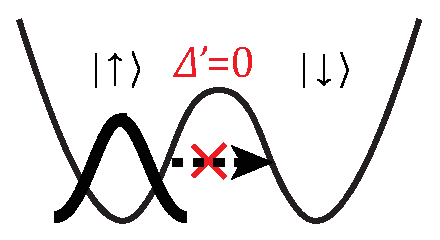
\includegraphics[height=3.7cm]{localization.eps}
	\caption{局在転移。トンネル振幅$\Delta'=0$となりトンネル効果が全く起こらず、状態が左右いずれかに局在している。}
	\label{fig:localization}
\end{figure}

スーパーオーミック散逸($s>1$)では、常に有効トンネル振幅は有限となり、
\begin{eqnarray}
	\Delta_{\mathrm{eff}} &=& \Delta e^{-F}, \\
	F &\equiv&\frac{1}{2}\int_{0}^{\infty}d\omega\frac{I(\omega)}{\omega^2} = \alpha \Gamma(s-1)
	\label{super_ohmic_kurikomi}
\end{eqnarray}
となる。一方、サブオーミック散逸($0<s<1$)では、$\Delta/\omega_c \rightarrow 0$の極限では$\Delta_{\mathrm{eff}}=0$となる\cite{Leggett87}。
ただし、有限の$\Delta/\omega_c$に対しては、温度ゼロにおいて、ある臨界値$\alpha = \alpha_c$において
量子相転移の存在が知られている\cite{Vojta05}。ここで$\alpha_c$はスペクトル関数の指数$s$および
$\Delta/\omega_c$によって決まる臨界値である。
この量子相転移(局在転移)を解析することが、本研究の目的の1つである。ここで、断熱くりこみの結果

本研究では、熱コンダクタンスの近似解を計算するにあたって、$\Delta_{\mathrm{eff}}$が有限の値として求まる領域では$\Delta_{\mathrm{eff}}$を典型的な温度スケールとし、$\Delta_{\mathrm{eff}} \rightarrow 0$となる領域では$\Delta$を典型的な温度スケールとして採用する。

%==========================================================
\subsection{Sequential tunneling}

\begin{figure}[tb]
	\centering
	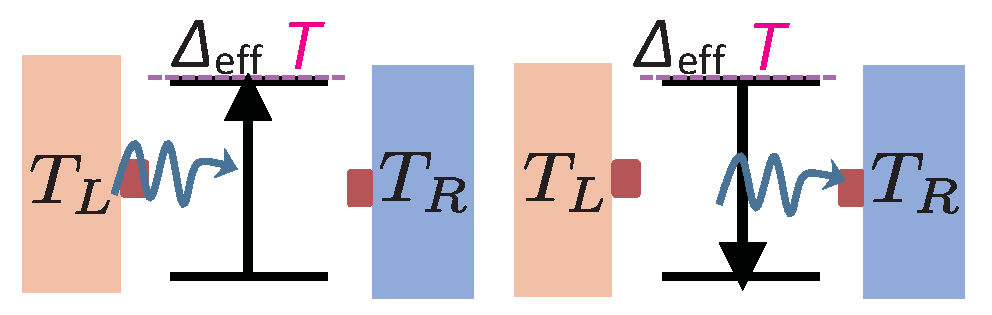
\includegraphics[height=3.5cm]{sequential_tunneling.eps}
	\caption{Sequential tunneling過程の模式図。温度$T$がエネルギー準位差$\Delta_{\rm{eff}}$に等しいため、このエネルギーを持つボゾンの吸収・放出の2つの過程によって輸送が起こる。}
	\label{fig:sequential_tunneling}
\end{figure}

二準位系と熱浴の間の結合が十分弱いときは、結合を摂動として取り扱うことができると期待される。
まず、二準位系と熱浴の間に結合がないときは、二準位系は量子トンネル効果によって基底状態$\ket{0}$と励起状態$\ket{1}$の間にエネルギー差$\Delta$が生じる。
次に熱浴の効果を2次摂動で取り入れると、熱浴から二準位系のエネルギー差$\Delta$に対応するエネルギーのフォノンが吸収・放出されることで熱輸送が行われる(図\ref{fig:sequential_tunneling})。この過程は確率的であり、マスター方程式によって記述される\cite{Ruokola11}が、輸送過程は吸収と放出の2つのステップから成り、輸送前後でフォノン(ボゾン)の位相情報は保たれていない点に留意すべきである。

ここでは簡単のため、応答スペクトル関数
\begin{eqnarray}
S(\omega) \equiv \frac{{\rm Im}[\chi(\omega)]}{\omega}
\end{eqnarray}
を利用した議論を行う
(この方法は、マスター方程式を解いて得られる結果と同じ結果を与える)。
二準位系と熱浴の間に結合がないとき、応答スペクトル関数$S(\omega)$は$\omega=\pm\Delta$にピークを持ったデルタ関数型の関数として
\begin{eqnarray}
	S(\omega) = \frac{\Delta}{\pi} \left[\delta(\omega-\Delta)+\delta(\omega+\Delta) \right]
\end{eqnarray}
と計算される。二準位系と熱浴の間の結合が弱ければ、同様に
\begin{eqnarray}
	S(\omega) \simeq A \left[\delta(\omega-\Delta_{\rm eff})+\delta(\omega+\Delta_{\rm eff})\right]
\end{eqnarray}
の形で応答スペクトル関数を近似できると期待される。実定数$A$はKramers-Kronigの関係式
\begin{eqnarray}
	\frac{1}{\pi}\int_{-\infty}^{\infty}d\omega S(\omega)&=&\frac{1}{\pi}\int_{-\infty}^{\infty}d\omega \frac{\mathrm{Im}[\chi(\omega)]}{\omega}\\
&=&\mathrm{Re}[\chi(0)]
	\label{Kramers-Kronig}
\end{eqnarray}
より$A=\pi\mathrm{Re}[\chi(0)]/2=\pi\chi_m/2$を満たす。ここで$\chi_m$は以下の式で定義される
二準位系の応答係数(二準位系をスピンとみなしたときの帯磁率)である。
\begin{eqnarray}
\chi_m \equiv \lim_{\epsilon \rightarrow 0} \frac{\langle \sigma_z \rangle}{\epsilon}
\label{chimdef}
\end{eqnarray}
量子トンネル振幅が$\Delta_{\rm eff}$の二準位系の帯磁率は$\chi_m = (2/\Delta_{\rm eff}) \tanh(\beta \Delta_{\rm eff}/2)$と計算できるので、式(\ref{exact_kappa})より
\begin{eqnarray}
	\kappa&\simeq& \frac{\pi\alpha\omega_c^{1-s}}{4}\frac{ \Delta_{\mathrm{eff}}^{s}}{2n(\Delta_{\mathrm{eff}})+1}\left[\frac{\beta\Delta_{\mathrm{eff}}/2}{\mathrm{sinh}{(\beta\Delta_{\mathrm{eff}}/2})}\right]^{2}
	\label{compare_ruokola2}
\end{eqnarray}
と求まる。ここで、$n(\omega)$はボーズ・アインシュタイン分布である。式(\ref{compare_ruokola2})の温度依存性は$\kappa\propto\beta^2e^{-\beta\Delta_{\mathrm{eff}}}$となっており、低温に向けて指数関数的に減少していく。
これは熱浴のフォノンの熱ゆらぎが小さくなるにつれて、系がエネルギー$\Delta_{\rm eff}$のフォノンを吸収する確率が急激に減少するからである。
$\Delta_{\rm eff}$は系を励起するのに必要なエネルギーであり、これより低温で輸送が急速に抑えられる現象は、量子ドット系におけるクーロンブロッケード現象に類似している。

Sequential tunnelingは二準位系と熱浴の結合が十分弱いときによい記述となるが、温度領域に制限がかかる。
まず温度が低くなると、次節で記述するcotunneling過程が優勢となる。
オーミック散逸では$\alpha<1$のときのみsequential tunnelingが起こる。
またサブオーミック散逸の場合は、温度が高くなると散逸が系のコヒーレンスを破壊してしまうので、
次々節で記述するincoherent tunnelingによる記述がよくなる。
一方、$s\geq2$のスーパーオーミック散逸のときには、結合の強度によらずsequential tunneling過程が
よい記述となる温度領域が存在するが、$1<s<2$のスーパーオーミック散逸では、量子力学的なマスター方程式から、デルタ関数型の応答スペクトルによるsequential tunnelingの仮定が成り立たなくなるクロスオーバー温度$T\simeq\Delta_{\rm eff}\alpha^{-1}(\omega_c/\Delta_{\rm eff})^{s-1}$が存在することが示唆されている\cite{Leggett87}。

%==========================================================
\subsection{Cotunneling}

系のエネルギースケール$\Delta_{\mathrm{eff}}$よりも十分低温の領域における
熱コンダクタンスの近似的表式を求める。ただし、ここでは局在転移は起こらない場合を考え、$\Delta_{\rm eff}\neq0$とする。
この温度領域では熱コンダクタンスの解析表式(\ref{exact_kappa})の積分において、$(\beta\omega/2)/\mathrm{sinh}(\beta\omega/2)$の因子により、低温では$\omega$がゼロ近傍の寄与が支配的である。
さらに、$T=0$において応答関数$\mathrm{Im}[\chi(\omega)]$と二準位系の帯磁率$\chi_m$を関係付ける、以下の関係式が成り立つことが知られている\cite{Sassetti90}。
\begin{eqnarray}
	 \lim_{\omega \to 0+} \frac{\mathrm{Im}[\chi(\omega)]}{\omega^{s}}=2\pi\alpha\left(\frac{\chi_m}{2}\right)^{2}
	 \label{shiba}
\end{eqnarray}
ここで帯磁率$\chi_m$は式(\ref{chimdef})で定義される。
この関係式は、オーミック散逸のときには近藤模型でフェルミ流体理論を考察して得られる斯波関係式\cite{Shiba75,Tsvelick83,Okiji87}と等価である。
以下では式(\ref{shiba})を一般化斯波関係式を呼ぶ。
一般化斯波関係式(\ref{shiba})は$T=0$で成り立つ関係式であるが、ここで$T\ll\Delta_{\rm{eff}}$を満たす有限温度でも成り立つと仮定すると、この領域の熱コンダクタンスの近似解は式(\ref{exact_kappa})から
\begin{eqnarray}
	\kappa&\simeq& \frac{\pi\omega_c^{s-1}\chi_m^2}{8}\int_{0}^{\omega_{c}}d\omega  I_L(\omega)I_R (\omega)\left[\frac{\beta\omega/2}{\sinh{(\beta\omega/2)}}\right]^{2}
	\label{compare_ruokola1}
\end{eqnarray}
と求まる。この表式はcotunneling近似で得られる表式とほぼ同じである\cite{Ruokola11}。
ただし、通常の摂動論に基づくcotunneling過程の計算では、上式の$\chi_m$が$2/\Delta$に
置き換わっているのに対し、式(\ref{compare_ruokola1})は$\chi_m$を通して断熱くりこみの効果も
含まれるため、適用範囲が広い。

さらに式(\ref{compare_ruokola1})の温度依存性を露わにすると
\begin{eqnarray}
	\kappa\simeq \frac{\pi\omega_c^{1-s}}{8}\left( \alpha \chi_m \right)^2 F(s)T^{2s+1}
	\label{cond_lowtemp},\\
	F (s)=\int_{0}^{\beta\omega_{c}}dx  x^{2s}\left[\frac{x/2}{\sinh({x/2})}\right]^{2}
\end{eqnarray}
となる。
ここで、帯磁率の温度依存性についても考慮する必要があるが、
オーミック散逸やスーパーオーミック散逸の場合は熱浴中の全ボゾンの効果を$\Delta$にくりこむことができるので、単純に$\Delta_{\rm eff}$の準位差を持った孤立した二準位系の帯磁率を計算すれば良い。
この結果、簡単な計算により低温領域で$\chi_m=2\mathrm{tanh(\beta\Delta_{\mathrm{eff}}/2)}/\Delta_{\mathrm{eff}}$と求まる。
これより、低温領域における熱コンダクタンスの温度依存性は$\kappa\propto T^{2s+1}$となることがわかる。
一方、サブオーミック散逸では帯磁率$\chi_m$の解析的な計算はスーパーオーミックのように孤立した二準位系に落とし込めないため容易では無い。
そこで本研究では数値計算によって得られる$\chi_m$を使って解析を行う。

\begin{figure}[tb]
	\centering
	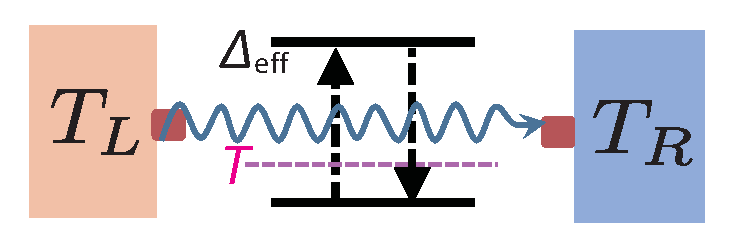
\includegraphics[height=3.5cm]{cotunneling.eps}
	\caption{Cotunneling過程の模式図。二準位系のエネルギー準位差$\Delta_{\rm{eff}}$に比べて温度$T$が非常に小さいため、本来ボゾンは吸収されないはずだが、バーチャルな励起によるボゾン輸送が起こる。}
	\label{fig:cotunneling}
\end{figure}

Cotunneling過程を使った熱輸送の模式図を図\ref{fig:cotunneling}に示す。低温領域ではエネルギー分裂$\Delta_{\mathrm{eff}}$に比べて温度$T$が十分小さいため、sequential tunneling過程において熱浴からフォノンを吸収して二準位系を励起する過程が抑制される。しかし、より高次の摂動(系と熱浴の結合の4次摂動)まで考えると、系のバーチャルな励起によって引き起こされるcotunneling(図\ref{fig:cotunneling})によって熱が輸送される。
Cotunneling過程では、位相の情報を保ったまま1プロセスで熱が運ばれる点に留意すべきである。

Cotunneling領域は$\Delta_{\rm eff}$が有限となる場合であれば、任意の$s$, 任意の結合強度$\alpha$に対して、
低温領域でよい記述となる。一方、量子相転移によって局在転移が生じて、$\Delta_{\rm eff}=0$となる場合は、
cotunneling過程は生じず、常に次節のincoherent tunneling過程となる。

%==========================================================
\subsection{Incoherent  tunneling}

$T\gg\Delta_{\rm eff}$を満たす高温領域を考える。この領域では、熱ゆらぎによって二準位系の量子性(重ね合わせ状態)が壊され、結果として系は左右の井戸に局在した状態を確率的に行き来するようになる。
このとき、系は次の古典的なマスター方程式によって記述できる。
\begin{eqnarray}
	\frac{dP_+(t)}{dt}=\Gamma P_-(t) - \Gamma P_+(t) 
	\label{master_eq}
\end{eqnarray}
ここで、${P}_+$は粒子(スピン)が右の井戸に存在する(アップをとる)確率、${P}_-$は粒子(スピン)が左の井戸に存在する(ダウンをとる)確率で$P_++P_-=1$を満たす。このマスター方程式は、sequential tunneling過程で扱ったマスター方程式と比べて、左右の井戸に局在した状態を基底としている点が異なる。
$\Gamma$は単位時間あたりの遷移確率で、量子トンネル振幅$\Delta$に関する摂動計算(フェルミの黄金律)から
\begin{eqnarray}
	\Gamma&=&\left({\frac{\Delta}{2}}\right)^2\int_{-\infty}^{\infty}dt \ e^{-Q(t)},\label{Gamma} \\
	Q(t)&=&\int_{0}^{\infty}d\omega \frac{I(\omega)}{\omega^2}\left \{ \mathrm{coth\left(\frac{\beta \omega}{2}\right)[1-\mathrm{cos}(\omega t)]+\it{i} \ \mathrm{ sin}(\omega t)}\right \}
\end{eqnarray}
と求まる\cite{Leggett87}。
式(\ref{master_eq})を初期条件$P_+(0)=1$のもとで解くと、
揺動散逸定理を用いて応答スペクトル関数$S(\omega)$は
\begin{eqnarray}
	S(\omega)&=&\frac{2\Gamma/T}{\omega^2+4\Gamma^2}\simeq \frac{2\Gamma}{\omega^2T}
\end{eqnarray}
と求まり、高温領域$T\gg\Delta$では$S(\omega)\simeq 2\Gamma/\omega^2T$と近似できる。これを式(\ref{exact_kappa})に代入すると、この領域における近似解は
\begin{eqnarray}
	\kappa&\simeq&\frac{\alpha\omega_c^{1-s}}{2}G(s)\Gamma T^{s-1} 
	\label{sub_ohmic_hightemp}
\end{eqnarray}
と求まる。ここで
\begin{eqnarray}
	G(s)=\int_{0}^{\beta \omega_c}dx\, x^{s-1}\left[\frac{x/2}{\sinh{(x/2)}}\right]^{2}
\end{eqnarray}
とおいた。$\Gamma$の具体的な計算に関しては、式(\ref{Gamma})における$Q(t)$の収束性から$s$の値によって場合分けする必要が生じる。オーミック散逸($s=1$)における$\Gamma$の計算は文献\cite{Weiss99}で行われており、この結果
\begin{eqnarray}
	\kappa\simeq\frac{\sqrt{\pi}\Gamma(\alpha)}{4\Gamma(\alpha+1/2)}\frac{\Delta^2}{\omega_c}\left(\frac{\pi T}{\omega_c}\right)^{2\alpha-1}
	\label{ohmic_incoherent}
\end{eqnarray}
となることがわかる。また、サブオーミック散逸($s<1$)における$\Gamma$は鞍点法によって計算でき、この結果は
\begin{eqnarray}
	\Gamma&=&\frac{\Delta^2}{4}e^{-\frac{\beta \Lambda_1}{4}}\sqrt{\frac{\pi \beta}{\Lambda_2}},\\
	 \Lambda_1&=&8T\alpha\Gamma(s-1)+16T\alpha\Gamma(s-1)\left(\frac{T}{\omega_c}\right)^{s-1}(2-2^{s-1})\zeta(s-1),\\
	 \Lambda_2 &=&T\left(\frac{T}{\omega_c}\right)^{s-1}2\alpha(2^{s+1}-1)\Gamma(s+1)\zeta(s+1)
\end{eqnarray}
となる\cite{Weiss99}。ここで、$\zeta(x)$はゼータ関数である。これより、サブオーミック散逸におけるincoherent tunneling過程の熱コンダクタンスの近似解は
\begin{eqnarray}
	\kappa\simeq\frac{\alpha\omega_c^{1-s}}{2}G(s)\frac{\Delta^2}{4}e^{-\frac{\beta \Lambda_1}{4}}\sqrt{\frac{\pi \beta}{\Lambda_2}}T^{s-1} 
	\label{sub_ohmic_hightemp}
\end{eqnarray}
と書ける。
\begin{figure}[tb]
	\centering
	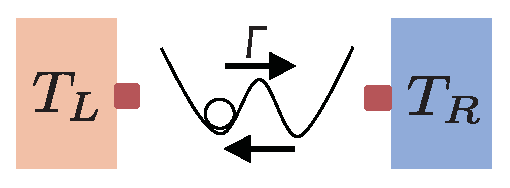
\includegraphics[height=3.5cm]{incoherent_tunneling.eps}
	\caption{Incoherent tunneling過程の模式図。単位時間あたりのトンネル確率$\Gamma$で左右の井戸のトンネルが起こり、これに揺さぶられたボゾンが輸送される。}
	\label{fig:incoherent_tunneling}
\end{figure}

Incoherent tunneling過程の模式図を図\ref{fig:incoherent_tunneling}に示す。
この過程では、系の波動関数は常に左右の井戸のどちらかに局在しており、
左右の井戸の間を遷移確率$\Gamma$で行き来する運動が生じることによって、
熱浴から別の熱浴へと熱輸送が起こる。
Incoherent tunnelingでは、系の位相情報は常に失われており、
輸送前後でフォノンのコヒーレンスは失われていている。

Incoherent tunneling過程は散逸の影響が強い状況で生じる。具体的には
$0<s<2$の高温側で生じる。特に量子相転移による局在転移が
生じると、任意の温度領域で熱輸送はincoherent tunneling過程で記述される。
一方、$s\geq2$のスーパーオーミック散逸では、incoherent tunneling過程は生じない。
これは、式(\ref{Gamma})で決まる遷移確率の式で、積分が発散することから示唆される。